%% ----------------------------------------------------------------------
\chapter{Planning the follow-up: the audit and the next observations}
\label{ch:followup}

A run ends with an FPP and an NFPP, but the more useful question for an
observer is: \emph{which observation would change them most?} The pipeline
answers it at the end of every run, and the audit repeats the answer with its
own checks.

\section{The idea}
TRICERATOPS splits the probability over its scenarios (Chapter~2). The FPP is
the sum of the false-positive scenarios, and each kind of follow-up
observation can rule out a known group of them:

\begin{longtable}{@{}p{0.27\textwidth}p{0.3\textwidth}p{0.36\textwidth}@{}}
\toprule
\textbf{Observation} & \textbf{Scenarios it can remove} & \textbf{How}\\
\midrule\endhead
Ground photometry with a separate aperture on the target and on each nearby star & NTP, NEB, NEBx2P on stars wider than the seeing (\code{--ground-fwhm}, default 3$''$) & The star that shows the dip is the host. One good transit is enough.\\
High-resolution imaging (speckle, adaptive optics) & bound companions (PEB, PEBx2P, STP, SEB, SEBx2P), background stars (DEB, DEBx2P, BTP, BEB, BEBx2P), neighbours closer than the seeing & A contrast curve; it sees companions outside its inner working angle (\code{--hires-iwa}, default 0.1$''$).\\
Reconnaissance spectroscopy (2--3 epochs, $\sim$1~km\,s$^{-1}$) & EB and EBx2P on the target; bright bound companions & A stellar companion on the target gives a radial-velocity amplitude of km\,s$^{-1}$; a bright companion shows its own set of lines (SB2), also closer than imaging can resolve.\\
Transits in two or more filters & scenarios in which the dip comes from, or is diluted by, a star of another colour & A planet on the target has the same depth in every band.\\
\bottomrule
\end{longtable}

For every observation the pipeline computes what the FPP and NFPP would become
if the scenarios it addresses were ruled out:
\[
\mathrm{FPP}' = \frac{\sum_{\rm FP\ kept} p_i}{\sum_{\rm all\ kept} p_i},
\qquad
\mathrm{NFPP}' = \frac{\sum_{\rm NTP,NEB\ kept} p_i}{\sum_{\rm all\ kept} p_i},
\]
where $p_i$ are the pooled scenario probabilities of the run. It then
searches the shortest combination of observations that would bring FPP and
NFPP below the validation limits.

\section{Best case and typical outcome}
No observation removes everything it addresses. The guide therefore gives two
numbers per observation:
\begin{description}
\item[Best case:] every scenario the observation addresses is ruled out.
\item[Typical:] only the part an observation of that kind usually reaches:
\begin{itemize}
\item \emph{imaging}: the bound companions wider than the inner working angle.
With the separation distribution of Sun-like binaries (Raghavan et al.\ 2010)
and 0.1$''$ at 373~pc (37~au) that is about half of them; background stars:
95\%;
\item \emph{spectroscopy}: 70\% of the bright companions (their velocity can
coincide with that of the target);
\item \emph{multi-band transits}: the share of possible companions whose
colour differs enough to change the depth by more than 20\% between the two
filters (below); background stars, whose colour is unknown: 50\%;
\item \emph{ground photometry}: all of the resolved neighbours.
\end{itemize}
\end{description}
These typical fractions are reasonable assumptions, not measurements. They
rank the observations; they do not predict their outcome. And an observation
can also \emph{find} a false positive: if the ground light curve shows the dip
on the neighbour, the candidate is a nearby eclipsing binary, whatever the
numbers said.

\section{The colour test in detail}
If the dip comes from star X and is diluted by star Y, the observed depth in a
band is the true depth times the share of X in the light of that band:
\[
\delta_{\rm band} = \delta_X \,\frac{F_{X,{\rm band}}}{F_{X,{\rm band}} + F_{Y,{\rm band}}} .
\]
The share changes with the band when X and Y have different temperatures.
The pipeline approximates both stars by blackbodies (g$'$ at 0.48~$\mu$m,
z$'$ at 0.91~$\mu$m, TESS at 0.80~$\mu$m) and estimates the temperature of a
companion from its mass with a main-sequence relation
($T_{\rm eff} \approx 5772~{\rm K}\,(M/M_\odot)^{0.6}$):
\begin{itemize}
\item \textbf{STP, SEB} (dip on the companion): a redder companion makes the
dip deeper in z$'$ than in g$'$ (ratio below 1);
\item \textbf{PEB} (dip on the target, diluted by the companion): only a small
effect, a few percent;
\item \textbf{planet on the target}: ratio 1, apart from limb darkening.
\end{itemize}
How large the effect is depends on the companion, which the TESS data hardly
constrain. The pipeline therefore runs over all possible companions (mass
ratio 0.1--1, flat distribution), keeps those bright enough to produce the dip
at all (for STP a planet of at most two Jupiter radii, for SEB an eclipse of at
most 100\%), and counts the share that changes the depth by more than 20\%.
The best fit of the last TRICERATOPS run is shown as an example together with
the precision that a band test would need (three times the depth error must
fit in the depth difference).

\section{Companions that Gaia already excludes: MOLUSC}
\label{sec:molusc}

\subsection*{Why}
Several false-positive scenarios of TRICERATOPS need an unresolved
\emph{bound companion} of the target: PTP and PEB (the companion dilutes
the dip), STP and SEB (the dip is on the companion). Without other
information TRICERATOPS uses a general prior: how often stars of this mass
have a companion, and with which masses and separations (Moe \& Di~Stefano
2017). For many nearby stars that prior is too pessimistic: Gaia has
observed them for years, and a bright companion at the right distance would
have shown up. MOLUSC (\emph{Multi-Observational Limits on Unseen Stellar
Companions}, Wood, Mann \& Kraus 2021, AJ~162, 128) turns those
non-detections into a list of the companions that are still allowed. It
costs no telescope time.

\subsection*{How MOLUSC works}
\begin{enumerate}
\item \textbf{Simulate.} It draws a large number of companions (typically
$10^6$) for the target: mass ratio $q$ uniform between 0 and 1, a log-normal
period distribution (Raghavan et al.\ 2010), and random eccentricity,
inclination, orientation and orbital phase. Each simulated star has
exactly \emph{one} companion.
\item \textbf{Predict what each companion would have done}, with the
stellar models of Baraffe et al.\ (2015) for its brightness:
\begin{itemize}
\item \emph{Gaia astrometry (RUWE).} A companion at roughly 0.1--1$''$
makes the photocentre wobble and raises the RUWE (renormalised unit weight
error) of the Gaia solution. MOLUSC predicts the RUWE for every simulated
companion and rejects those whose prediction is clearly larger than the
observed value.
\item \emph{Gaia imaging.} A companion bright enough and far enough from the
star (beyond about 1$''$) would be a separate Gaia source.
\item \emph{Optional:} a high-resolution contrast curve (speckle, AO) and
radial-velocity measurements. With RVs, close companions (a few au and
less) can be excluded as well.
\end{itemize}
\item \textbf{Keep the survivors.} The file \code{<prefix>_kept.csv} lists
the companions that none of the data would have seen.
\end{enumerate}
The rejections are probabilistic (a companion is rejected with the
probability that it would have been detected), so a run with $10^6$
companions gives smooth distributions.

\subsection*{How the pipeline uses it}
\begin{enumerate}
\item \textbf{Run MOLUSC.} A copy with a few small fixes (newer SciPy/NumPy, a VizieR fallback) is
in the folder \code{MOLUSC} (see \code{README_pipeline.txt}). For each target a
short script gives the coordinates and the mass, e.g.\ for L~279-94:
\begin{lstlisting}
bash MOLUSC/run_molusc_L27994.sh       # in WSL, about 10 min
# -> TIC100796276_molusc/L27994_N1000000_kept.csv
\end{lstlisting}
MOLUSC needs the Gaia archive; when it does not answer (for instance while
it is closed for the DR4 release), the same Gaia DR3 values are read from
VizieR.
\item \textbf{Give the file to the pipeline:} GUI tab \emph{Field},
``MOLUSC companions file'' (\code{--molusc-file}) and ``MOLUSC: companions
generated'' (\code{--molusc-n}, the number MOLUSC simulated).
\item \textbf{What happens inside.} TRICERATOPS(+) takes the mass ratios of
the MOLUSC companions for the first draws of the PTP, PEB, STP and SEB
scenarios, and treats the remaining draws as ``no companion''. Two details
matter:
\begin{itemize}
\item It keeps only companions whose orbit never comes closer than 10~au to
the star (periastron $a(1-e) > 10$~au). Planets are rare in such close
binaries (Moe \& Kratter 2021), so TRICERATOPS assumes they do not exist
there.
\item The prior probability of a companion then becomes (number of
companions in the file)/(number of TRICERATOPS draws, $10^6$). Used as is,
the FPP would depend on how many companions one happened to simulate in
MOLUSC, and a file with more than $10^6$ survivors would crash
TRICERATOPS. The pipeline therefore resamples the survivors so that this
probability equals the MOLUSC survival fraction times an assumed
multiplicity (\code{--molusc-multiplicity}, default 1: every star has a
companion, the conservative choice).
\end{itemize}
The log lists the numbers: companions generated, kept, kept beyond 10~au,
the resulting prior, and their mass-ratio distribution. The audit names
the companion prior that was used (\emph{Evaluation}).
\end{enumerate}

\subsection*{Limitations}
\begin{itemize}
\item \textbf{It removes only what Gaia could have seen.} Companions very
close to the star (periastron $\lesssim$1~au) hardly change the RUWE and are
not resolved; without RV data they all survive. That they do not count in
the FPP is the \emph{assumption} that planets avoid close binaries, not a
measurement. A result that relies on MOLUSC should say so, and spectroscopy
(RVs or a second set of lines) is the observation that tests it.
\item \textbf{The RUWE is not only a binary indicator.} Variability, a
nearby source or a poor fit also raise it; a high RUWE makes MOLUSC reject
\emph{fewer} companions, which is safe. A RUWE that is low by chance would
make it reject too many.
\item \textbf{Models and distributions.} The companion population
(Raghavan), the stellar models (BHAC15, default age 5~Gyr) and the RUWE
calibration of the MOLUSC tables are assumptions; for very young or
evolved stars they matter.
\item \textbf{One companion per star.} Triples are not simulated. The
multiplicity (fraction of stars that have a companion at all) is not part
of MOLUSC; the pipeline uses 1 unless told otherwise, which overestimates
the companion probability (about a quarter of M dwarfs have one,
Winters et al.\ 2019).
\item \textbf{Different versions, different answers.} TRICERATOPS 1.1.0
treats the MOLUSC companions differently from the TRICERATOPS+ version
used here; the Zenodo note on L~279-94 obtains FPPs between 0.003 and 0.042
depending on such choices. Report the FPP with the companion model.
\item \textbf{Not a replacement for high-resolution imaging.} MOLUSC shows
that the companions which would invalidate the planet are \emph{unlikely};
an image or RVs show whether one is \emph{there}.
\end{itemize}


\section{Where to find it}
\begin{itemize}
\item at the end of the log, section \emph{Next observations};
\item in \code{recommendations_<tic>.txt} and in \code{summary_<tic>.json}
(\code{recommendations});
\item on the page \emph{Next observations} of the audit report
(Figure~\ref{fig:audit-next}), together with the advice of the audit's own
tests.
\end{itemize}

\section{The audit}
\code{triceratops_audit.py} reads an output folder and tries to break the
claim of the run, with deterministic checks only (no language model). The GUI
starts it with the button \emph{Audit run} on the tab \emph{Results} or from
the menu \emph{Tools}; it writes \code{audit_<tic>.pdf}, \code{.txt} and
\code{.json} and opens the PDF. The input files are never changed.

The report has four parts:
\begin{enumerate}
\item \textbf{Skeptic}: 17 tests with PASS, WARN, FAIL or NA, each with its
evidence, the file and line it comes from, and an advice (ephemeris,
single events, depth consistency, odd/even, secondary eclipse, shape and
density, dilution, centroids, neighbours, Monte-Carlo convergence,
sensitivity, ground data, multi-band colours and TRICERATOPS+
(Section~\ref{sec:multiband}), provenance of the input depth, and two
independent recomputations from the saved light curves, which leave out the
sectors the pipeline excluded and the transits of masked candidates);
\item \textbf{Next observations} (this chapter);
\item \textbf{Evaluation}: every claim of the run with its source;
\item \textbf{Recomputation}: the audit's own fold and per-sector depths.
\end{enumerate}
A FAIL does not change the pipeline's verdict; it marks a claim that needs a
closer look before the result is reported.

\begin{figure}[p]
\centering
\includegraphics[page=3,height=0.86\textheight,trim=0 25mm 0 0,clip]{audit_65344135.pdf}
\caption{Audit of TIC~65344135 (run of 12~November 2026), page \emph{Next
observations}. Ground photometry with separate apertures removes the
neighbour (FPP $0.391 \rightarrow 0.026$); spectroscopy or a colour test then
removes most of the rest.}
\label{fig:audit-next}
\end{figure}
